\documentclass[../thesis.tex]{subfiles}

\begin{document}

To reach into confined spaces robot arms must be thin, long, and maneuverable.
A thin robot may have small actuators with limited torque such that the joints cannot support the weight of the outstretch cantilevered arm.
However confined spaces are filled with places to rest for support, and contact forces can compensate for low joint torque. 
Robot motion planners that take advantage of support enable new capabilities for long thin arms.

This chapter considers motion planning for a robot arm that may experience contact forces.
The motion planner's goal is to output a trajectory of joint torques that will start with the robot arm in an initial configuration in joint space, and end with the end effector in a specified location.
Each joint can only apply a limited torque, and the trajectory must respect these limits.
The arm experiences forces due to gravity, inertial, friction, and also interaction with the environment.
This dynamics model is described in detail in section \ref{sec:robot_dynamics}.
Contact forces can be helpful by balancing out gravity, or detrimental by blocking a desired motion.
Contact forces prove difficult due to their large but local effect.


Section \ref{sec:trajectory_optimization} describes a solution to the motion planning task that uses trajectory optimization and is strongly based on Contact Invariant Optimization \cite{Mordatch2012}.
The problem formulation includes a function that assigns a cost to each trajectory, and uses the gradient of this cost function to incrementally improve the trajectory.
Typically a trajectory is penalized for large joint torques and for not reaching the goal, however that formulation provides insufficient gradient information when contacts are involved.
The more accurate dynamics model is augmented, making it less accurate but better conditioned for optimization.

Section \ref{sec:sample_planning} describes a sampled-based planner capable of using contact forces, and again alterations are made to handle the thin contact manifold.







%% \section{Related Work}
\section{Robot Dynamics} \label{sec:robot_dynamics}

\begin{figure}
  \centering
  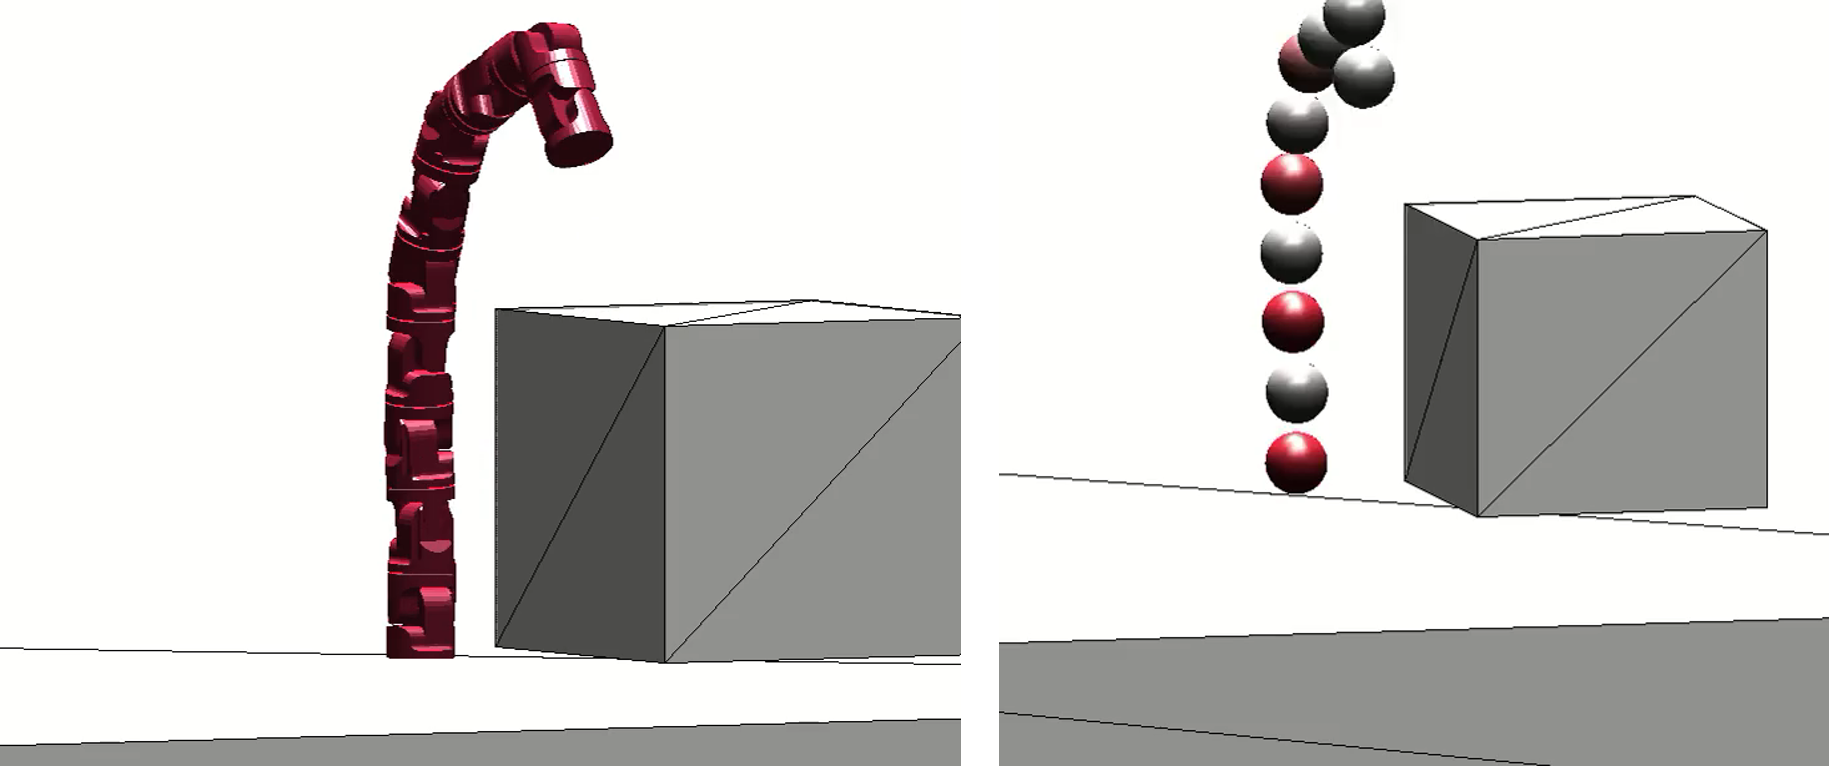
\includegraphics[width=.7\linewidth]{./Planning/sphere_approxmation.png}
  \caption{The visually accurate robot model (left) and the spherical approximation (right)}
  \label{fig:sphere_approxiamtion}
\end{figure}


When not in contact with the environment the robot model follows the manipulator arm equation \cite{murray1994mathematical}:
\begin{align}
  M(\theta)\ddot \theta + C(\theta, \dot\theta)\dot\theta + N(\theta, \dot\theta) = \tau
\end{align}
$M$ and $C$ are determined through the robot's known mass characteristics.
$N$ includes both gravity and frictional terms.
In practice $M, C,$ and $N$ do not need precise estimation, because closed loop controllers on the robot can compensate for errors.

The robot arm has defined sections which may be in contact with the environment.
For simplicity in calculations, these contact sections are approximated by spheres, shown in Figure \ref{fig:sphere_approximation}.
The environment is modeled as a triangular mesh, and contact occurs when a contact section intersection the mesh.
The contact force is determined by a spring model, and so the magnitude is proportional to the penetration distance with direction pushing the section out of the environment.
The physical robot and environment are both constructed of metal, so while a large spring constant provides a more accurate model this also causes numerical instabilities.
Each trajectory is simulated as a series of discrete time steps, and a large spring constant will result in giant forces for even the slight penetration this discretization introduces.

%% Figure \ref{fig:ThinManifold} illustrates the region of 








\section{Trajectory Optimization} \label{sec:trajectory_optimization}

\begin{figure}
  \centering
  \begin{subfigure}[b]{0.24\linewidth}
    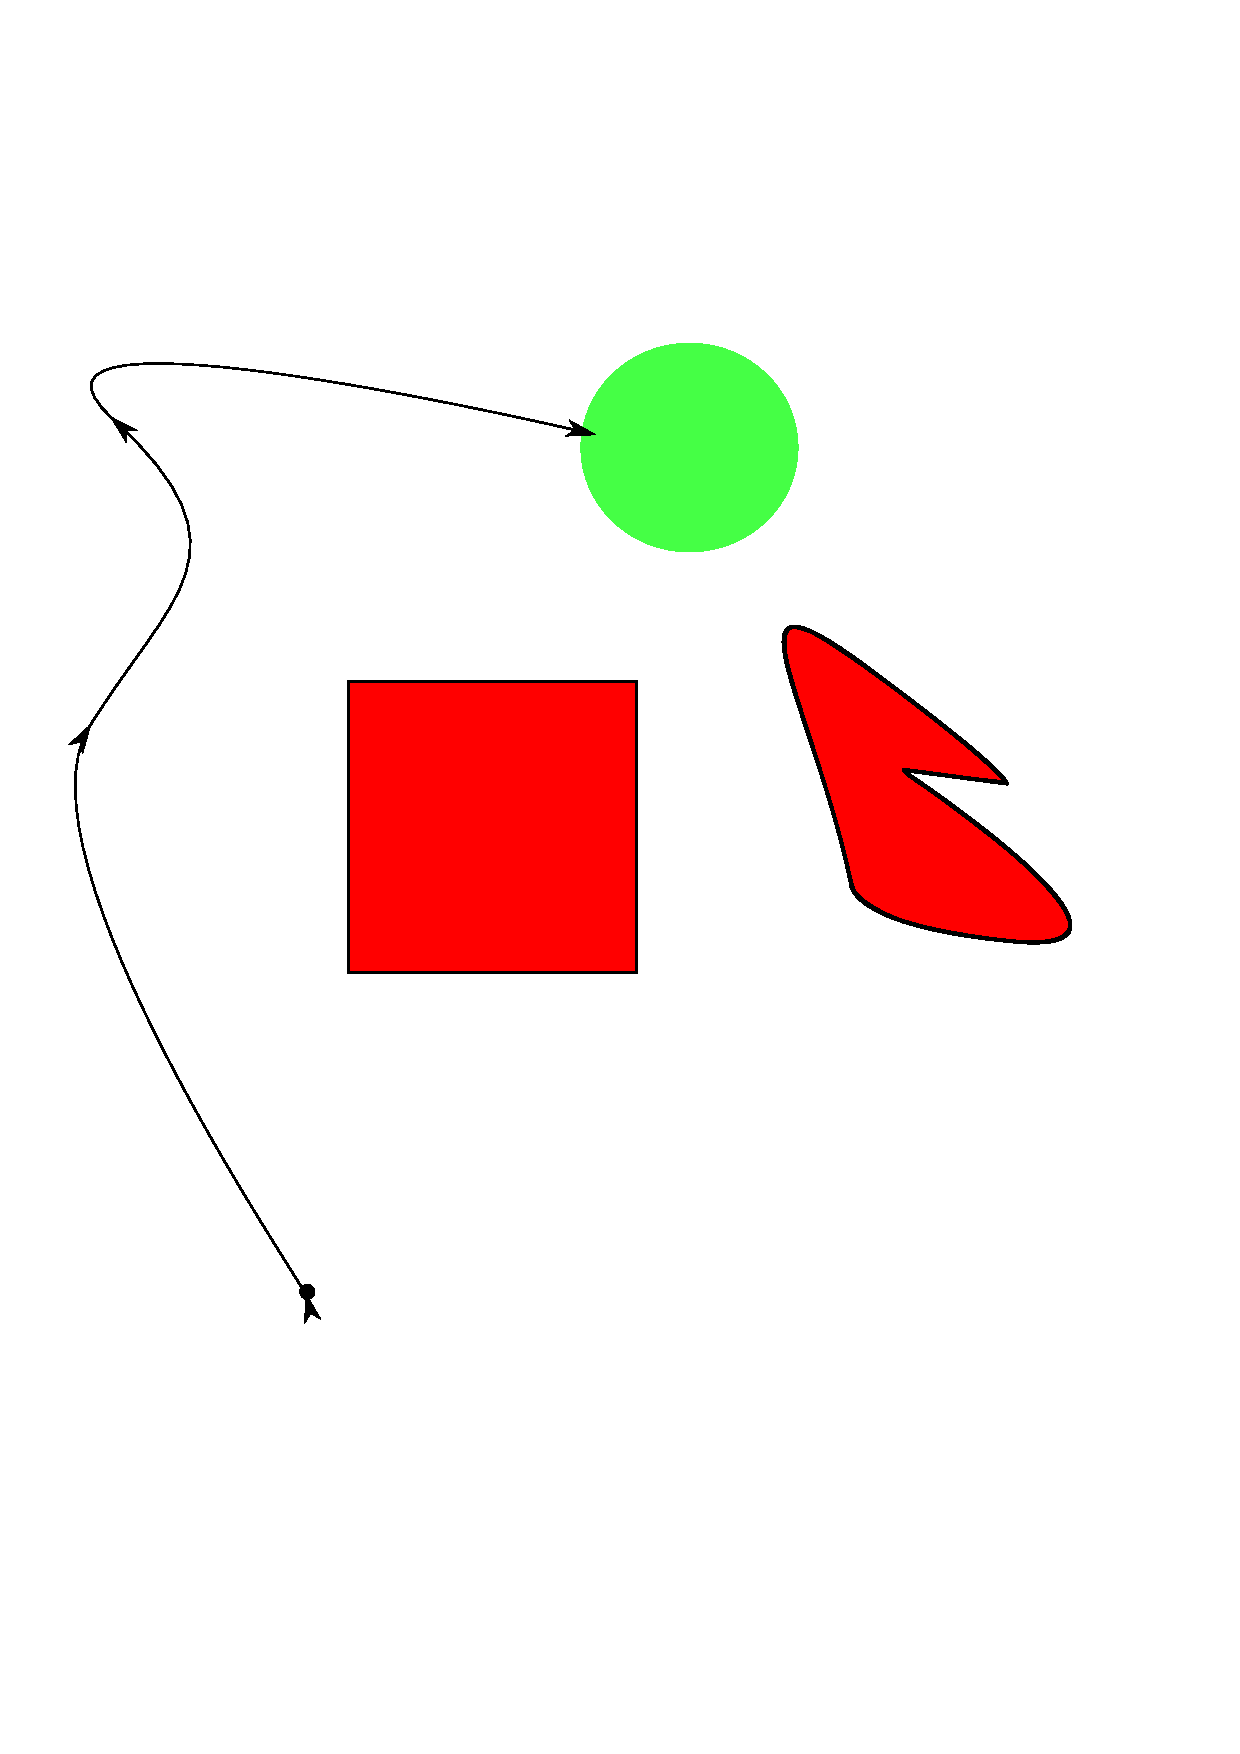
\includegraphics[width=\linewidth]{./Planning/trajectory_1.pdf}
  \end{subfigure}
  \hfill
  \begin{subfigure}[b]{0.24\linewidth}
    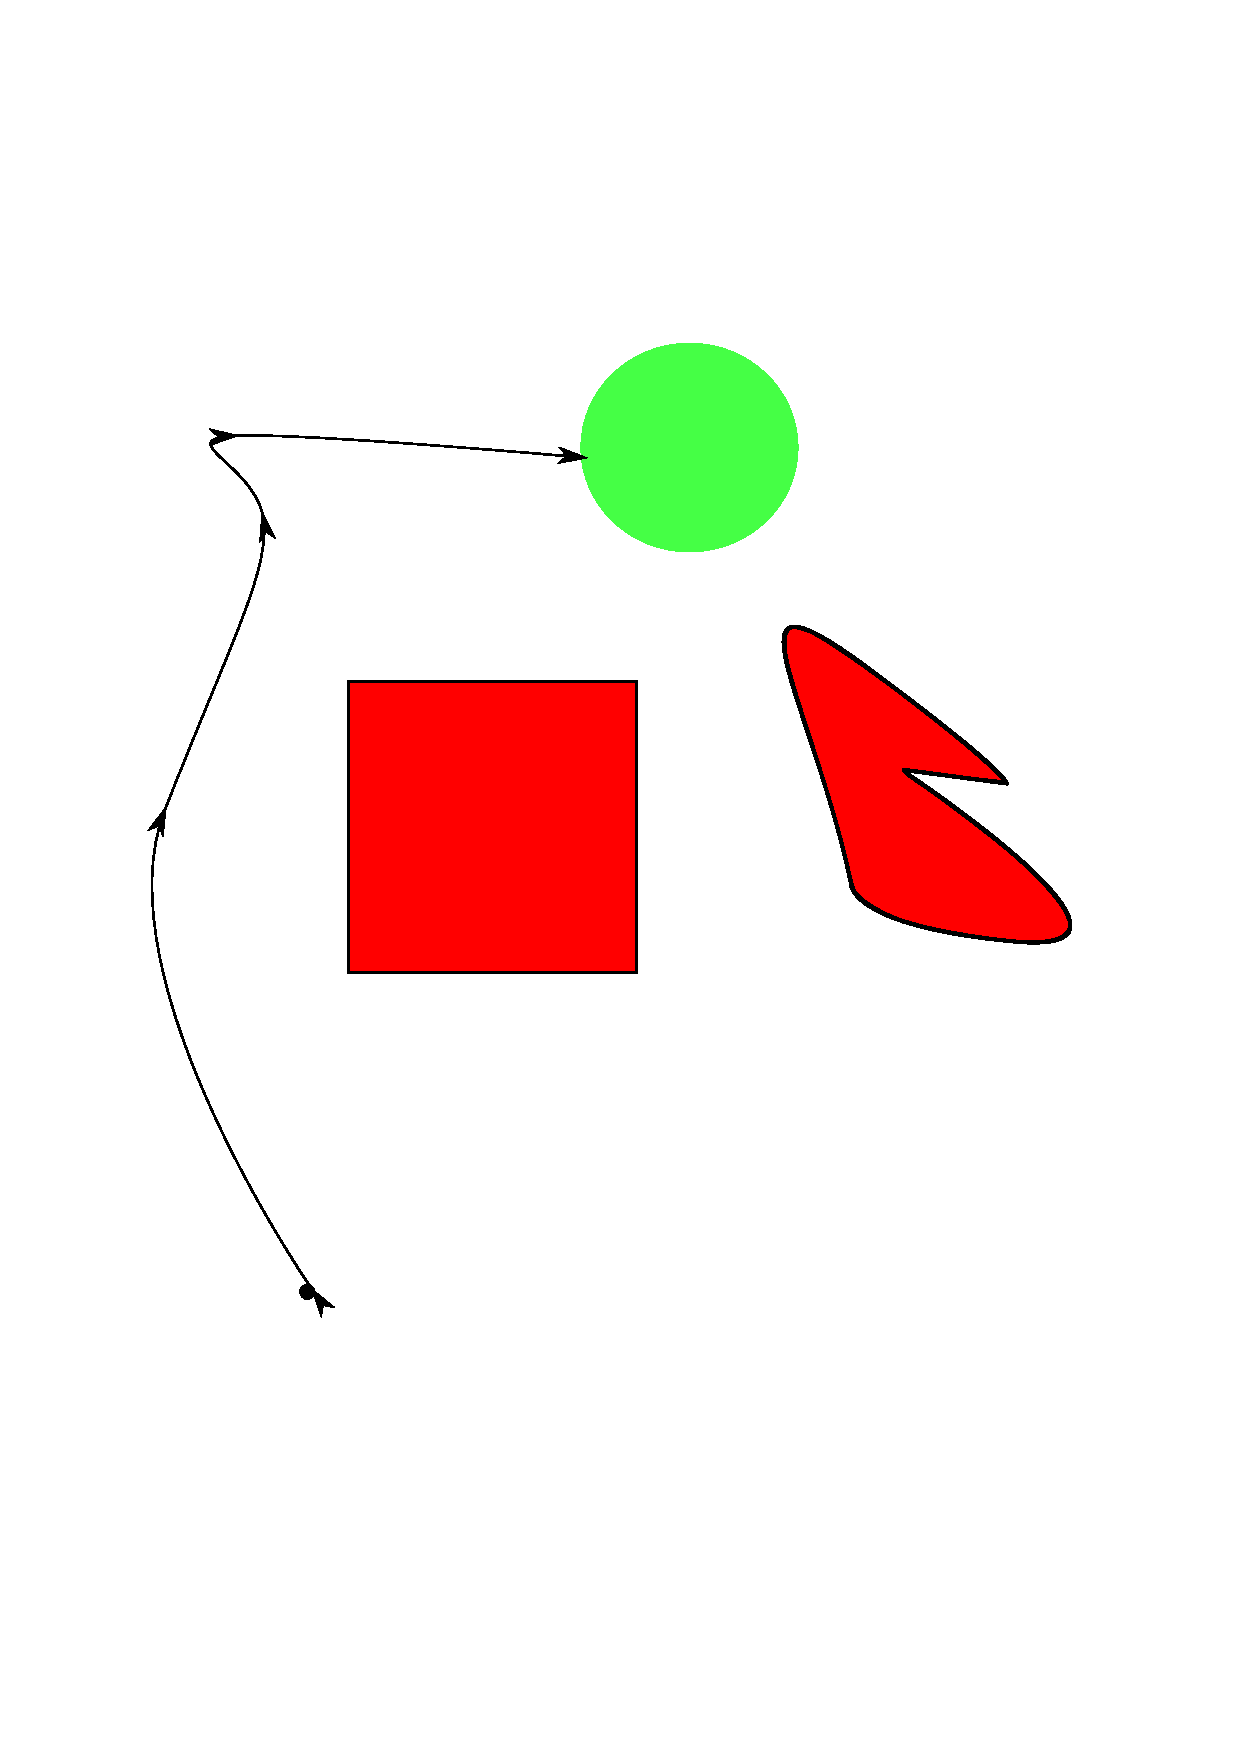
\includegraphics[width=\linewidth]{./Planning/trajectory_2.pdf}    
  \end{subfigure}
  \begin{subfigure}[b]{0.24\linewidth}
    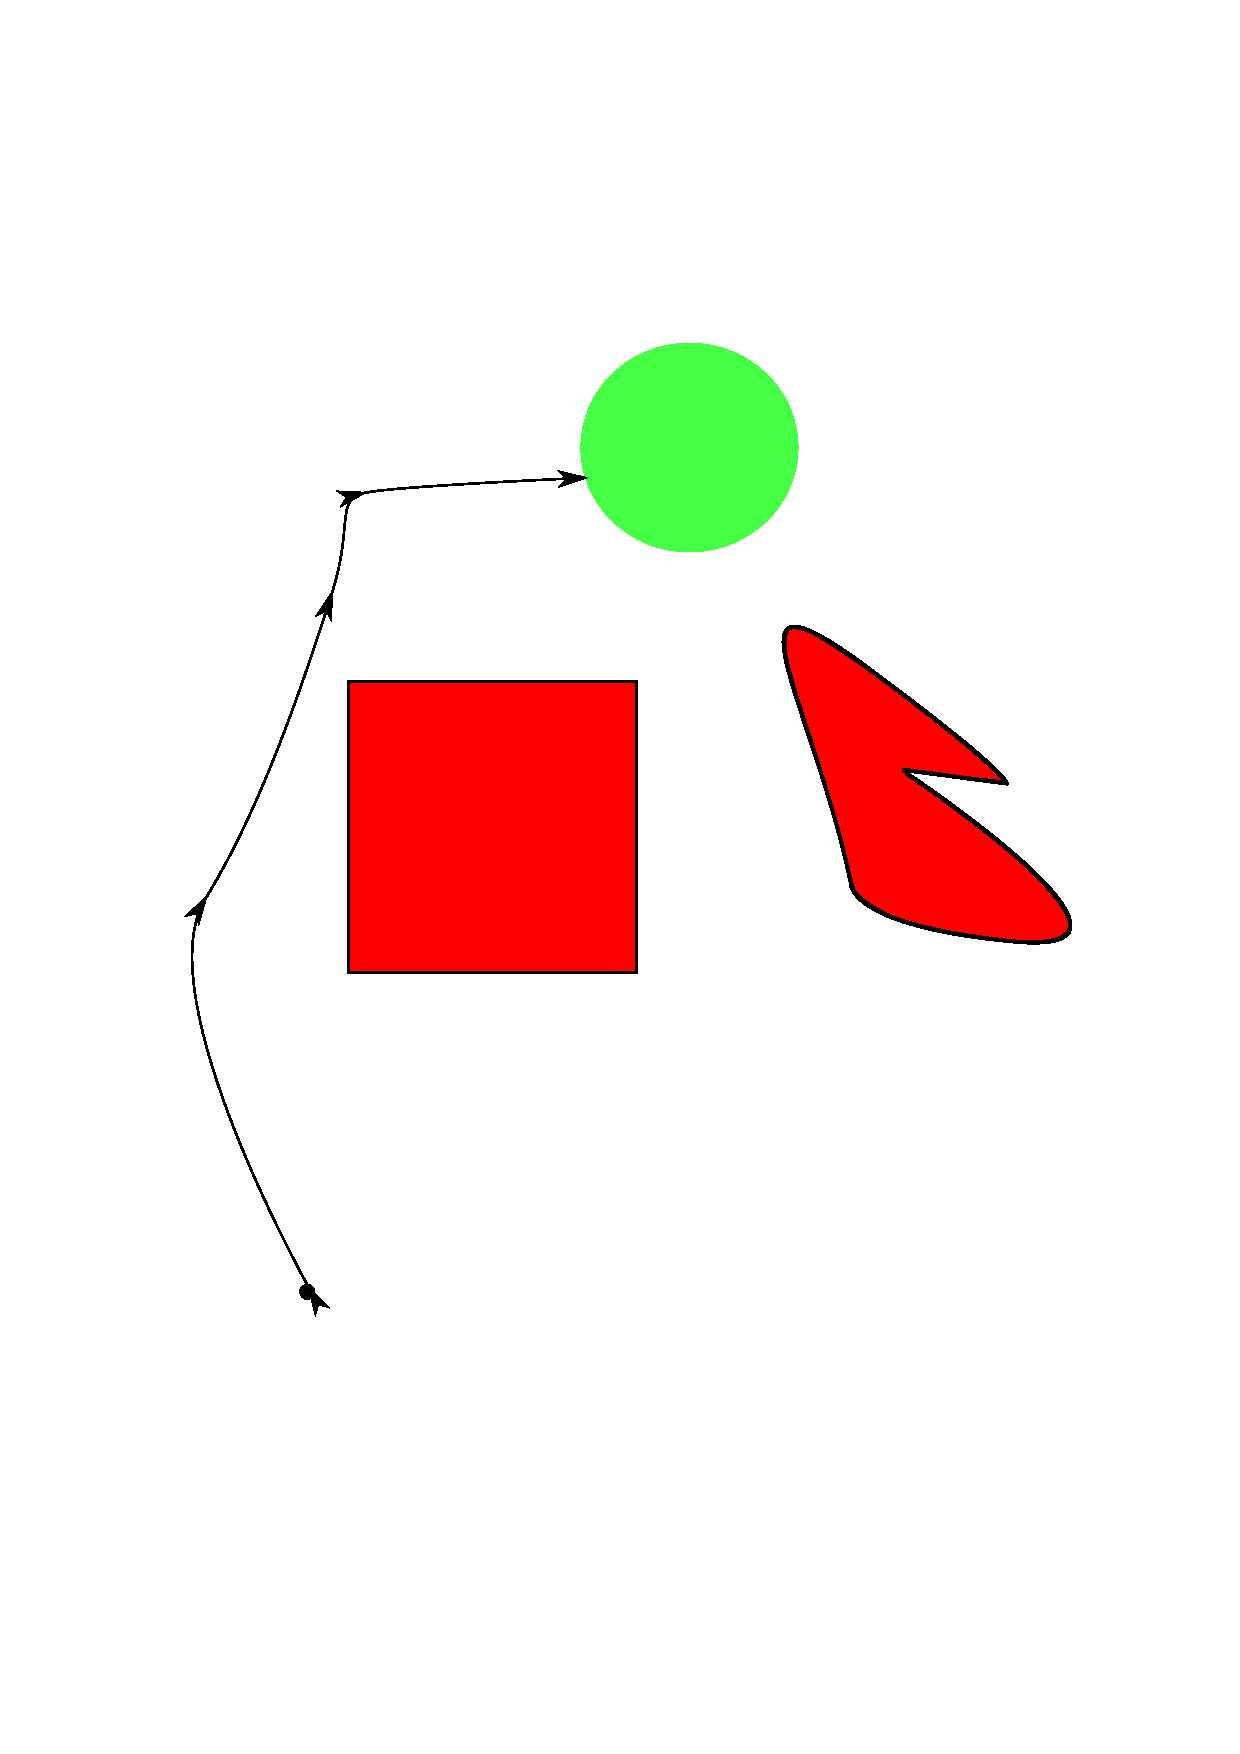
\includegraphics[width=\linewidth]{./Planning/trajectory_3.pdf}
  \end{subfigure}
  \hfill
  \begin{subfigure}[b]{0.24\linewidth}
    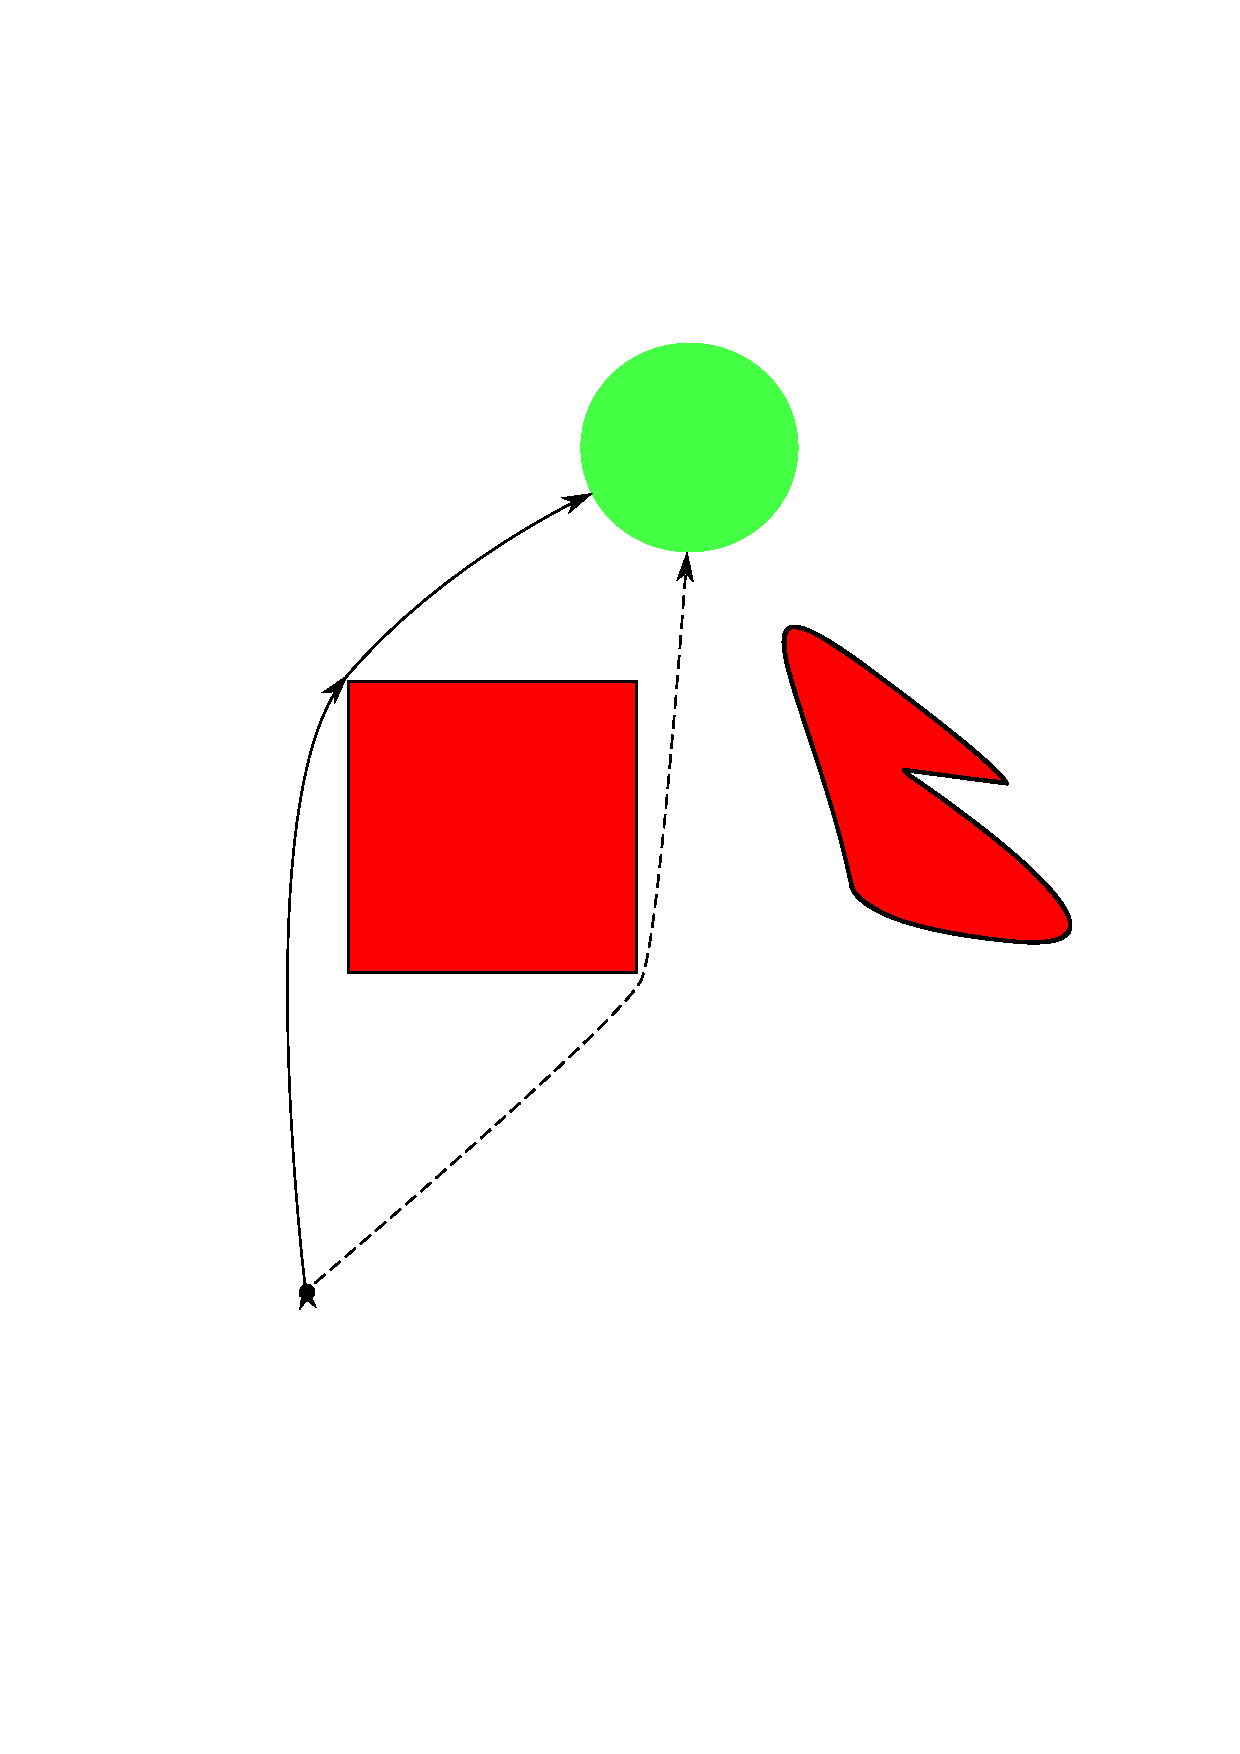
\includegraphics[width=\linewidth]{./Planning/trajectory_best.pdf}    
  \end{subfigure}
  
  \caption{Optimizing the shortest path trajectory from an initial path converges to a local best, but possibly misses the globally best solution.}
  \label{fig:TrajectoryOptimization}
\end{figure}


Trajectories for a robotic arm are created through trajectory optimization.
A trajectory $s$ is a discrete list of robot states $s_t$ at increasing points in time.
A state contains both the joint angles and joint velocities, though for sufficiently slow trajectories the velocities may be ignored.
To transition between timesteps, joint torques are calculated through inverse dynamics.

Since the trajectory requires maintaining low joint torques and reaching a goal point, it seems natural to define a cost function the penalizes joint torque and the distance from the goal:
\begin{align}
  L(s) = \sum ||\tau_{joint}||^2 + Cost_{task}
\end{align}
Figure \ref{fig:naive_cost} shows such a cost function for a single state for a simple robot arm with one movable base joint and one contact section on the end effector, with a goal position with the robot leaning to the right.
For simplicity, the dynamic forces are ignored and the only forces considered are gravity and contact.
Although the minimum of this cost function uses contact to reduce joint torque while reaching the goal, this cost function is poorly conditioned for gradient descent optimization.
Nearly all initializations will result in convergence to the local minimum with the wide basin of attraction at $\theta=0.1$.
Thus this cost function is augmented to be better suited for optimization.


\begin{figure}
  \centering
  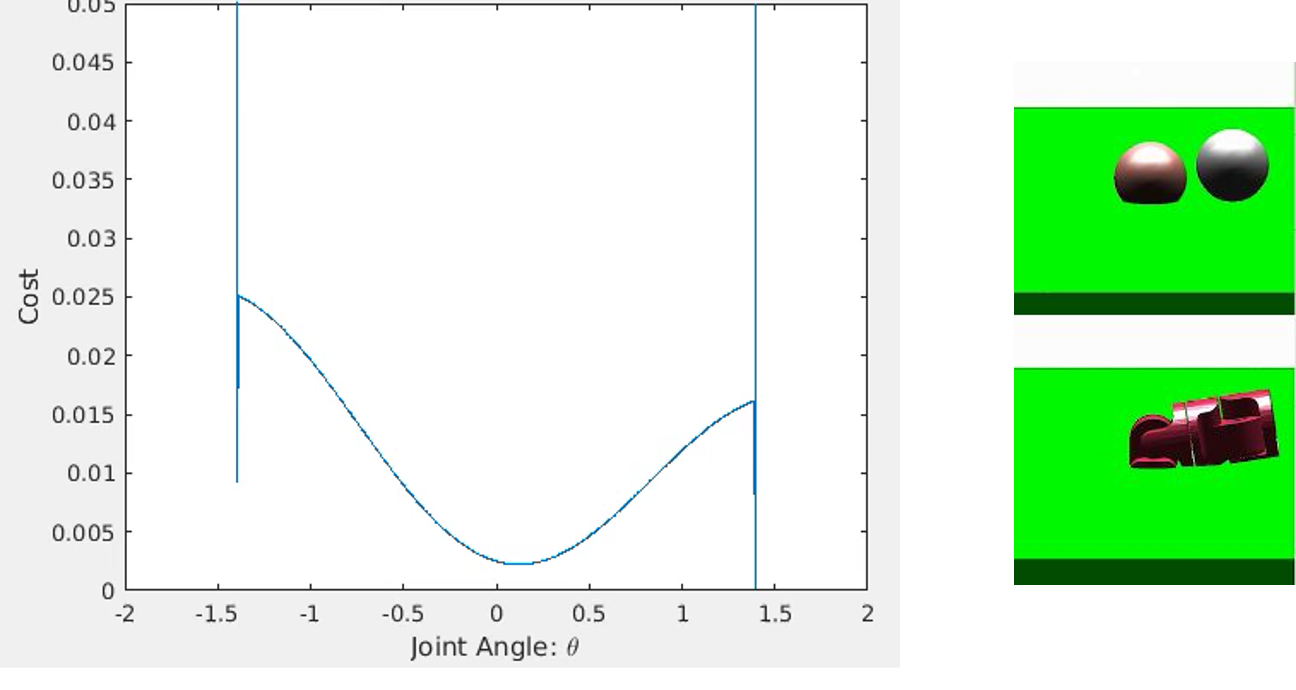
\includegraphics[width=\linewidth]{./Planning/naive_cost}
  \caption{Naive cost function, with sharp changes around contact locations}
  \label{fig:naive_cost}
\end{figure}
%% The formulation used in the paper follows from Mordatch's work \cite{Mordatch2012}.





\subsection{Auxiliary Variables}
The key approach used here is softening of contacts through the introduction of auxiliary variables which drastically smooth the cost function, at the expense of increasing the dimensionality of the state space.
Appended to each state $s_t$ is a set of auxiliary continuous variables $c_t$, one for each section of the robotic arm allowed to make contact with the environment.
The variables $c_t$ regulate the magnitude of the normal and frictional contact forces and will be described in detail.
%% These $c$ variables seem unnecessary as the forward kinematics specified by the joint angles $\theta$ determine the locations of the robot, and therefore determine the contacts between the robot and the environment.
Without this augmentations, slight changes in these joint configurations result in slight motion of the robot which may result in huge changes in contact forces.
Additionally without artificial terms in the cost function to model contact, the cost function is blind to potential contacts that may be close and useful.


\subsection{Smoothing the Cost Function}
The optimal solution $s^*$ is computed by minimizing the cost function of the form

\begin{align}
L(s) &= L_{Contact Violation} + L_{u} \\
&+ L_{Object Penetration} + L_{Goal}   
\end{align}
    
$L_{Object Penetration}$ and $L_{Goal}$ are straightforward, while the interplay between $L_{Contact Violation}$ and $L_u$ provide the interesting structure allowing the optimization to find paths which use supporting contacts.




\subsubsection{Cost $L_{Contact Violation}$}
Each section of the robot able to make contact has an associated variable $c_t > 0$ at each time step. $c$ intuitively represents the strength of the contact forces.
Since if the robot is not physically in contact with the world there will not be a contact force the cost $L_{Contact Violation}$ is introduced to penalize non-zero values of $c$ when the robot is not in contact. 
$$L_{Contact Violation} = \sum_t{\sum_i{c_{t,i} d_{t,i}}}$$
Non-zero values for $c$ are intentionally allowed when the robot is not in contact with the environment even though this is not physically realistic as this makes the cost function smooth.
However when optimizing $c_{t,i}$ will tend towards 0 unless the robot is in contact.

\begin{figure}
  \centering
  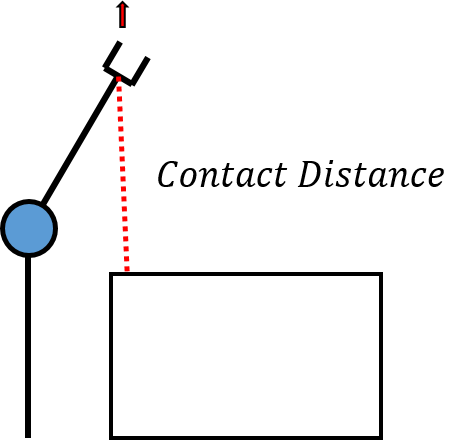
\includegraphics[width=.3\linewidth]{./Planning/contact_distance.png}
  \caption{Contact distance for the end effector section}
  \label{fig:contact_distance}
\end{figure}


\begin{figure}
  \centering
  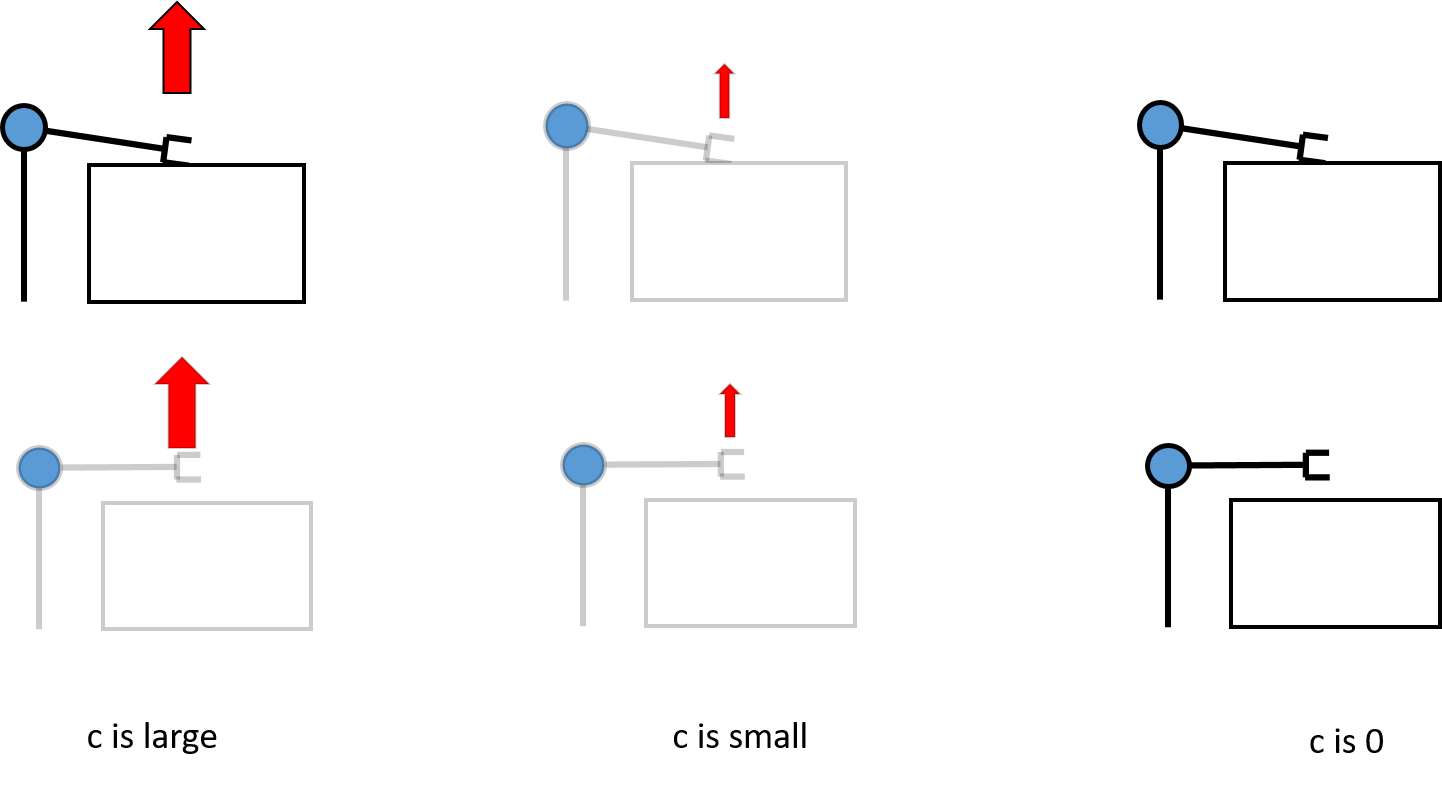
\includegraphics[width=.7\linewidth]{./Planning/ContactArms.png}
  \caption{Arm configuration and simulated (not realistic) contact forces for a variety of arm configurations and continuous contact variables}
  \label{fig:ContactArms}
\end{figure}

Figure \ref{fig:contact_distance} shows the contact distance for a section of a robotic arm. Since this distance is substantial, the magnitude of the associated contact variable will determine the contribution to cost. 

Figure \ref{fig:ContactArms} shows a robot arm in a variety of configurations and with several values of contact variables.
The transparent configurations are physically infeasible and suffer a $L_{Contact Violation}$ cost.
To ensure the final optimized trajectory is feasible, the contact violation cost is weighted highly towards the end of optimization, thus the optimization will not converge on any of the transparent configurations.




\subsubsection{Cost $L_u$}

\begin{figure}
  \centering
  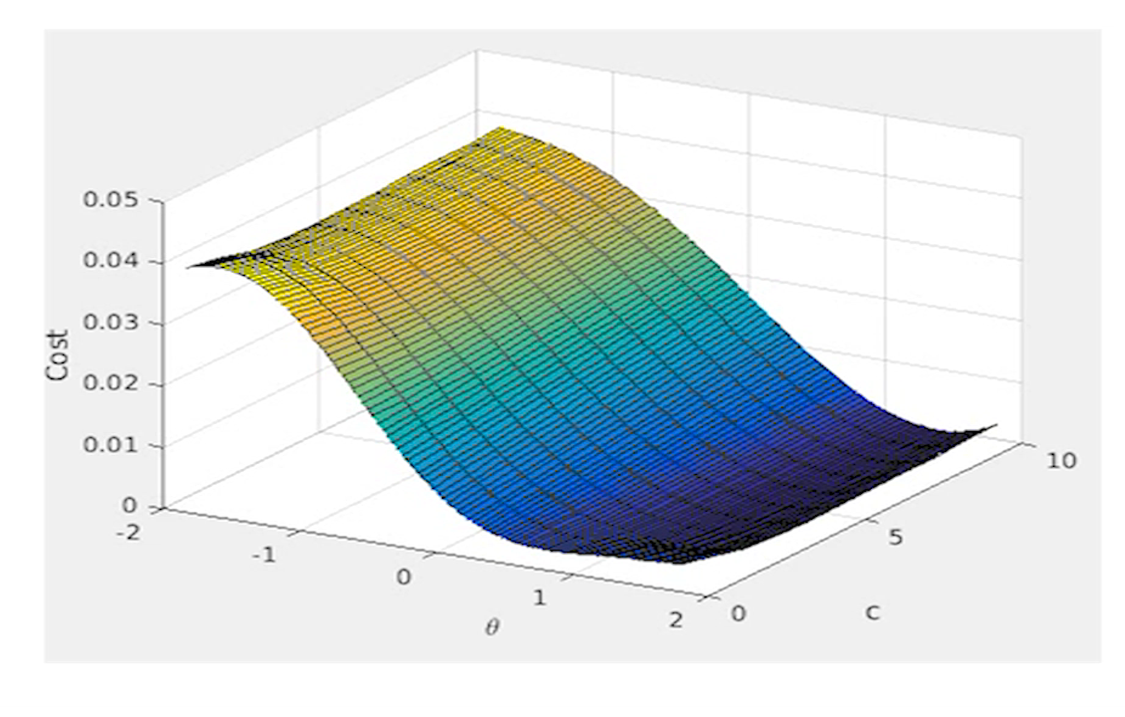
\includegraphics[width=.7\linewidth]{./Planning/augmented_cost.png}
  \caption{The cost function for the arm in Figure \ref{fig:naive_cost}, augmented with the auxiallary contact variable}
  \label{fig:augmented_cost}
\end{figure}


The cost $L_u$ penalizes the input torque necessary to follow the trajectory specified.
%% With no contacts these inputs could be calculated directly from the arm inverse dynamics.
As discussed the physical contact forces are extremely sensitive to robot configuration, so to soften the forces we instead compute the contact forces that minimize the joint torque.
When the trajectory is executed on the robot the joint controller will take responsibility for finding the slight adjustments in configuration to reach the desired contact forces.
The path planner does not have to worry about the minute adjustments for a model that will not match reality to that detail anyway.
Instead this path planner just needs to estimate the best contact forces possibly, according to the the following quadratic programming problem:
\begin{align}
f, u &= argmin_{\tilde{f}, \tilde{u}} ||J^T\tilde{f} + \tilde{u} - \tau_{Free}|| \\
&+ \tilde{f}^T W \tilde{f} + \tilde{u}^T R \tilde{u}
\end{align}

The input control regularization $R$ is chosen based on the desired penalization of joint inputs. The contact force regularization $W$ is dependent on the values of $c$, with 
$$W_{j,j} = \frac{1}{c_{i,t}^2 + 1}$$
If $c$ is large then the robot is in contact, the force regularization is small, so the contact force can be large. If $c$ is small the robot is not near any contact location, the force regularization is large, thus the contact force is heavily penalized and will be small.

Figure \ref{fig:ContactArms} shows a robot arm in a variety of configurations and with several values of contact variables.
The red arrows indicate the simulated contact force.
If the contact variable is large, a large force can be applied to reduce joint torques even when there is no physical contact.
This serves to reduce the cost due to joint torques.
The competing cost $L_{Contact Violation}$ prevents this contact variable from growing too large for infeasible contacts.


Figure \ref{fig:augmented_cost} shows this augmented cost function for the arm in Figure \ref{fig:naive_cost}.
The dimensionallity of this cost function has increased, yet now there is a strictly descending path from the local minima of the naive cost function, $\theta=0.1$, to the global minima.
The basin of attraction for the global minima has increased dramatically.




\subsubsection{Other Cost Terms}
$L_{Obstacle}$ penalizes penetration of the robot into the environment which is calculated using the robot forward kinematics.
For simplicity, the same simplified spherical model is resued here.
This addition is necessary since the artificial contact model created by $L_u$ and $L_{ContactViolation}$ no longer ensures obstacle penetration produces high joint torques.

\begin{align}
  L_{Obstacle} = \sum d_{ObstaclePenetration}
\end{align}

$L_{Goal}$ is a penalty on the distance from the robot end effector at the last state $s_T$ to the goal location.
\begin{align}
  L_{Goal} = ||EndEffector_T - goal||
\end{align}


\subsection{Initialization Challenges}
Although the cost function augmentation described above greatly improves the conditioning of the cost function with respect to contacts, in practical problems this cost function is still plagued with local minima.
As a simple example, consider the situation in Figure \ref{fig:local_min}, where most initial trajectories will result in the arm never reaching the goal ``X''.

Straightfoward initialization techniques include random initialization with random restarts, and linear joint angle interpolation between starting configuration and a configuration that achieves the goal.
These initializations work well in open environments, but poorly in confined spaces.
Thus a sample based planner is employed to provide a diversity of good initializations.

\begin{figure}
  \centering
  \begin{subfigure}[b]{0.4\linewidth}
    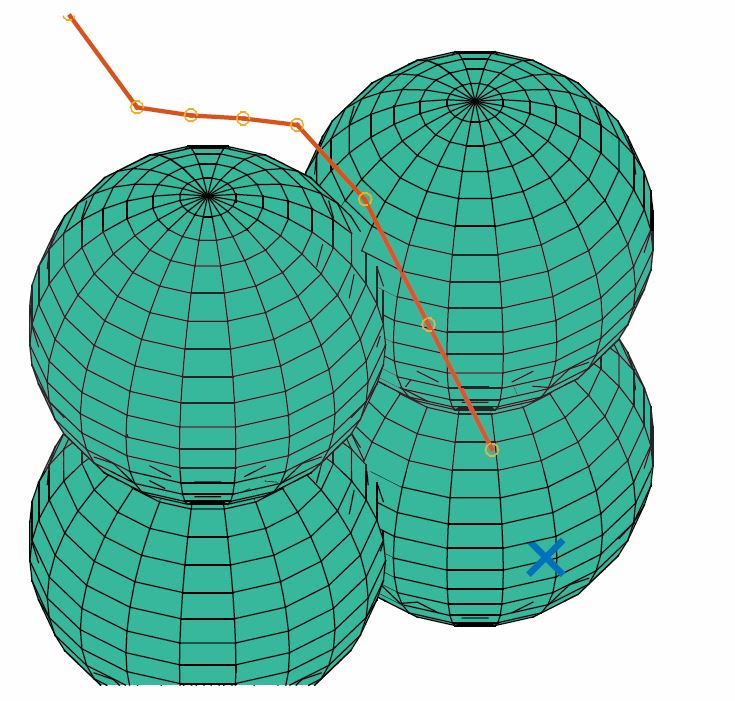
\includegraphics[width=\linewidth]{./Planning/Local.jpg}    
  \end{subfigure}
  \begin{subfigure}[b]{0.4\linewidth}
    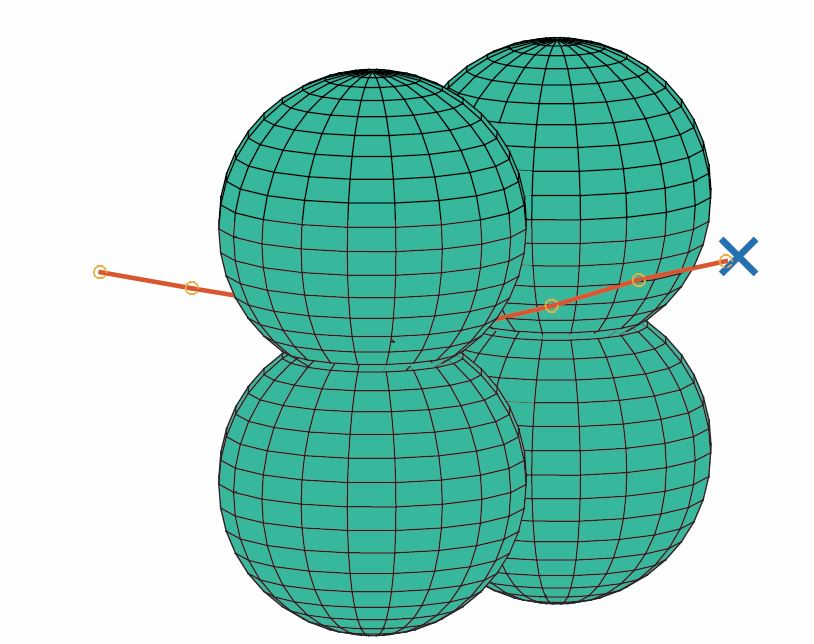
\includegraphics[width=\linewidth]{./Planning/global.jpg}    
  \end{subfigure}
  \caption{Trajectory optimization finding a local minimum (left) and the global minimum (right) for an arm attempting to reach the blue ``X''}
  \label{fig:local_min}
\end{figure}








\section{Sample Based Planning} \label{sec:sample_planning}
%% \subsection{RRTs and their variants}

\begin{figure}
  \centering
  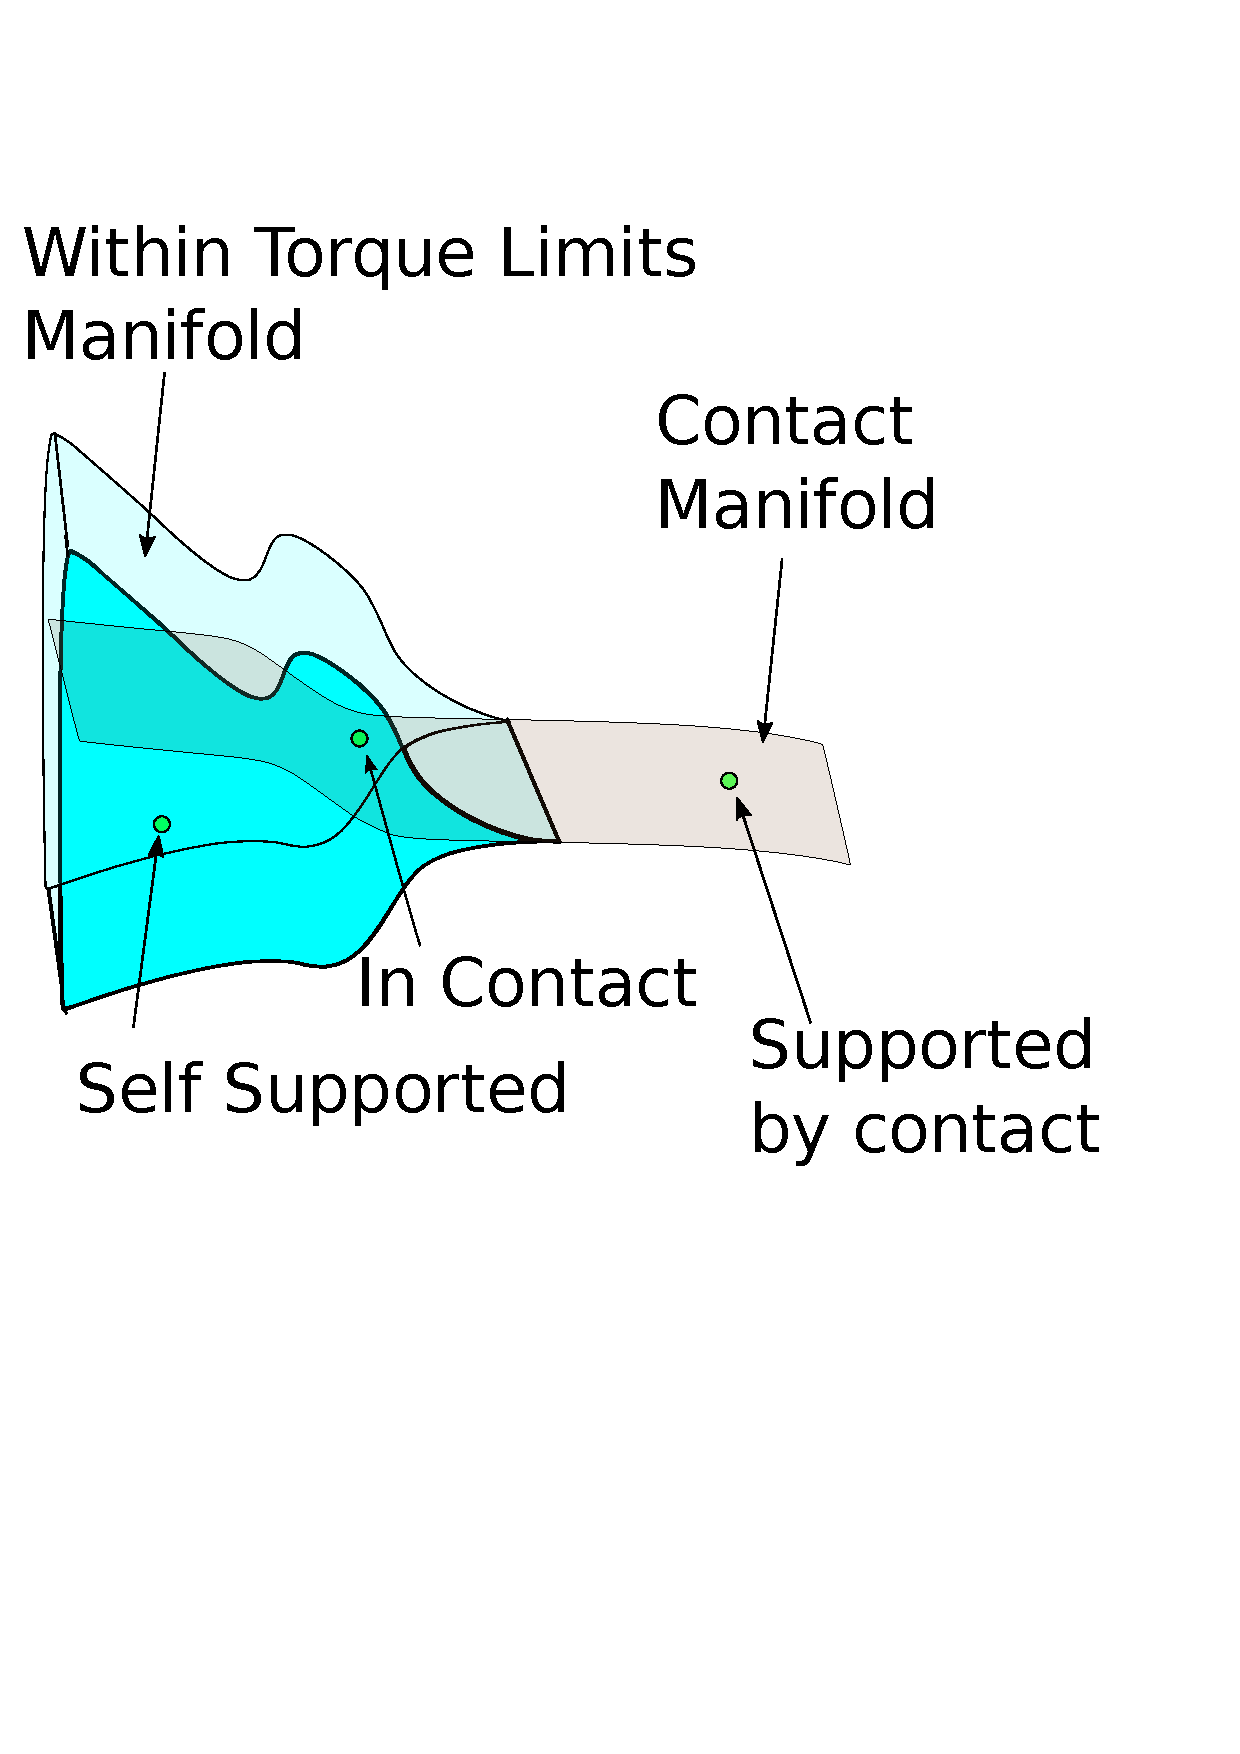
\includegraphics[width=.5\linewidth]{./Planning/thin_manifold.pdf}
  
  \caption{Illustration of valid configuration space for an arm potentially supported by contacts}
  \label{fig:ThinManifold}
\end{figure}

\subsection{Adaptation to Encourage Contacts}
Given:
\begin{align}
    &X \in \mathbb{R}^d:     &&\text{d-dimensional configuration space}\\
    &X_{obs} \subset X:      &&\text{obstacles in the configuration space}\\
    &X_{free} = X \setminus X_{obs}:   &&\text{free space}\\
    &x_{start} \in X_{free}:  &&\text{starting configuration}\\
    &X_{goal} \subset X_{free}: &&\text{set of goal configurations}\\
    &policy: X \times X \rightarrow TX &&\text{policy to goal, maps to tangent space (velocity).  Previous formulation was wrong, as need to be able to follow the policy to an arbitrary point in X, not just a goal configuration}
\end{align}

The goal is to find a path in $X_{free}$ from $x_{start}$ to $x_{goal} \in X_{goal}$.


\begin{algorithm}
\caption{$T=(V,E) \leftarrow$ policyRRT$(x_{start})$}\label{euclid}
\begin{algorithmic}[1]
\State $T \leftarrow$ InitTree($x_{start}$)
\While {GoalNotReached($T, X_{goal}$)}
\State $x_{rand} \in X \leftarrow$ Sample()
\State $x_{nearest} \leftarrow $ Nearest($T, x_{rand}$)
\State $T \leftarrow $ followPolicy$(x_{nearest}, x_{rand}, T$, extensionLimit)
\If {ExtensionSuccessful}
\State $T \leftarrow $ followPolicy$(x_{new}, x_{goal} \in X_{goal}, T, \infty)$
\EndIf
\EndWhile
\end{algorithmic}
\end{algorithm}

\begin{algorithm}
\caption{$T=(V,E) \leftarrow$ followPolicy$(x_{begin}, x_{end}, T$, iterLimit)}\label{euclid}
\begin{algorithmic}[1]
\State $T_{new} \leftarrow $ InitTree($x_{begin}$)
\State $x_{prev} \leftarrow x_{begin}$
\State $x_{new} \leftarrow $ policy($x_{prev}, x_{end}$)
\State $i \leftarrow 0$
\WhileNoDo{MovingTowardsGoal($x_{new}, T_{new}$) \textbf{and}}
\StatexIndent[2] Nearest($T, x_{new}$) == $x_{begin}$ \textbf{and}
\StatexIndent[2] i $<$ iterLimit
\algorithmicdo
\State $T_{new} \leftarrow $ AddNode($x_{new}, x_{prev}, T_{new}$)
\State $x_{prev} \leftarrow x_{new}$ 
\State $x_{new} \leftarrow $ policy($x_{prev}, x_{end}$)
\State $i \leftarrow i+1$
\EndWhile
\State $T \leftarrow $ AddTreeToTree($T_{new}, T, x_{begin}$)
\end{algorithmic}
\end{algorithm}

In many environments, it is relatively easy to compute a reactive policy that can make forwards progress towards a goal while avoiding collision with obstacles, such as a potential field approach, but such policies are prone to getting stuck in local minima/dead ends.  PolicyRRT is a variant of RRT that seeks to combine the efficient, goal directed trajectory generation of reactive policies with the ability of RRT to find paths around local minima/dead ends.  PolicyRRT fundamentally behaves like a standard RRT by growing a tree by iteratively extending towards a randomly sampled configuration from the nearest point in a search tree $T$.  PolicyRRT uses the reactive policy to move towards the random sample, potentially enabling the planner to avoid collisions with obstacles during the extension.  When PolicyRRT is successful in extending towards the sample (does not collide with an obstacle and does not get stuck in a local minima) it then follows the policy to extend towards the goal.  To avoid oversampling regions associated with local minima, when PolicyRRT extends towards a point from some vertex $v \in T$ PolicyRRT halts extension when the trajectory leaves the Voronoi cell of $v$.  Extension is also halted once the policy ceases to make progress (reaches a local minima) or exceeds a maximum number of iterations (only when extending towards $x_{rand}$?)

PolicyRRT is beneficial when a policy that would yield a path all the way from $x_{start}$ and $x_{goal}$ is difficult to find but finding a policy that can make some progress while avoiding obstacles, but may get stuck in local minima is relatively easy. An example of such a policy is a \textbf{potential field}: a cost function is constructed by placing attractors at the goals and repulsions at obstacles and the policy is to the gradient of this cost.  Potential fields are generally much simpler to compute than the minima-free navigation functions, but cannot be guaranteed to produce a path.  Augmenting the gradient descent policy with an RRT can help find paths out of any local minima.

Similarly augmenting an RRT with a reactive policy can assist in navigating narrow passages.  Because the policy will naturally flow through corridors PolicyRRT no longer requires drawing samples inside the narrow corridor itself, as drawing a sample from the far side may suffice to draw the policy through the corridor.

\begin{figure}
  \centering
  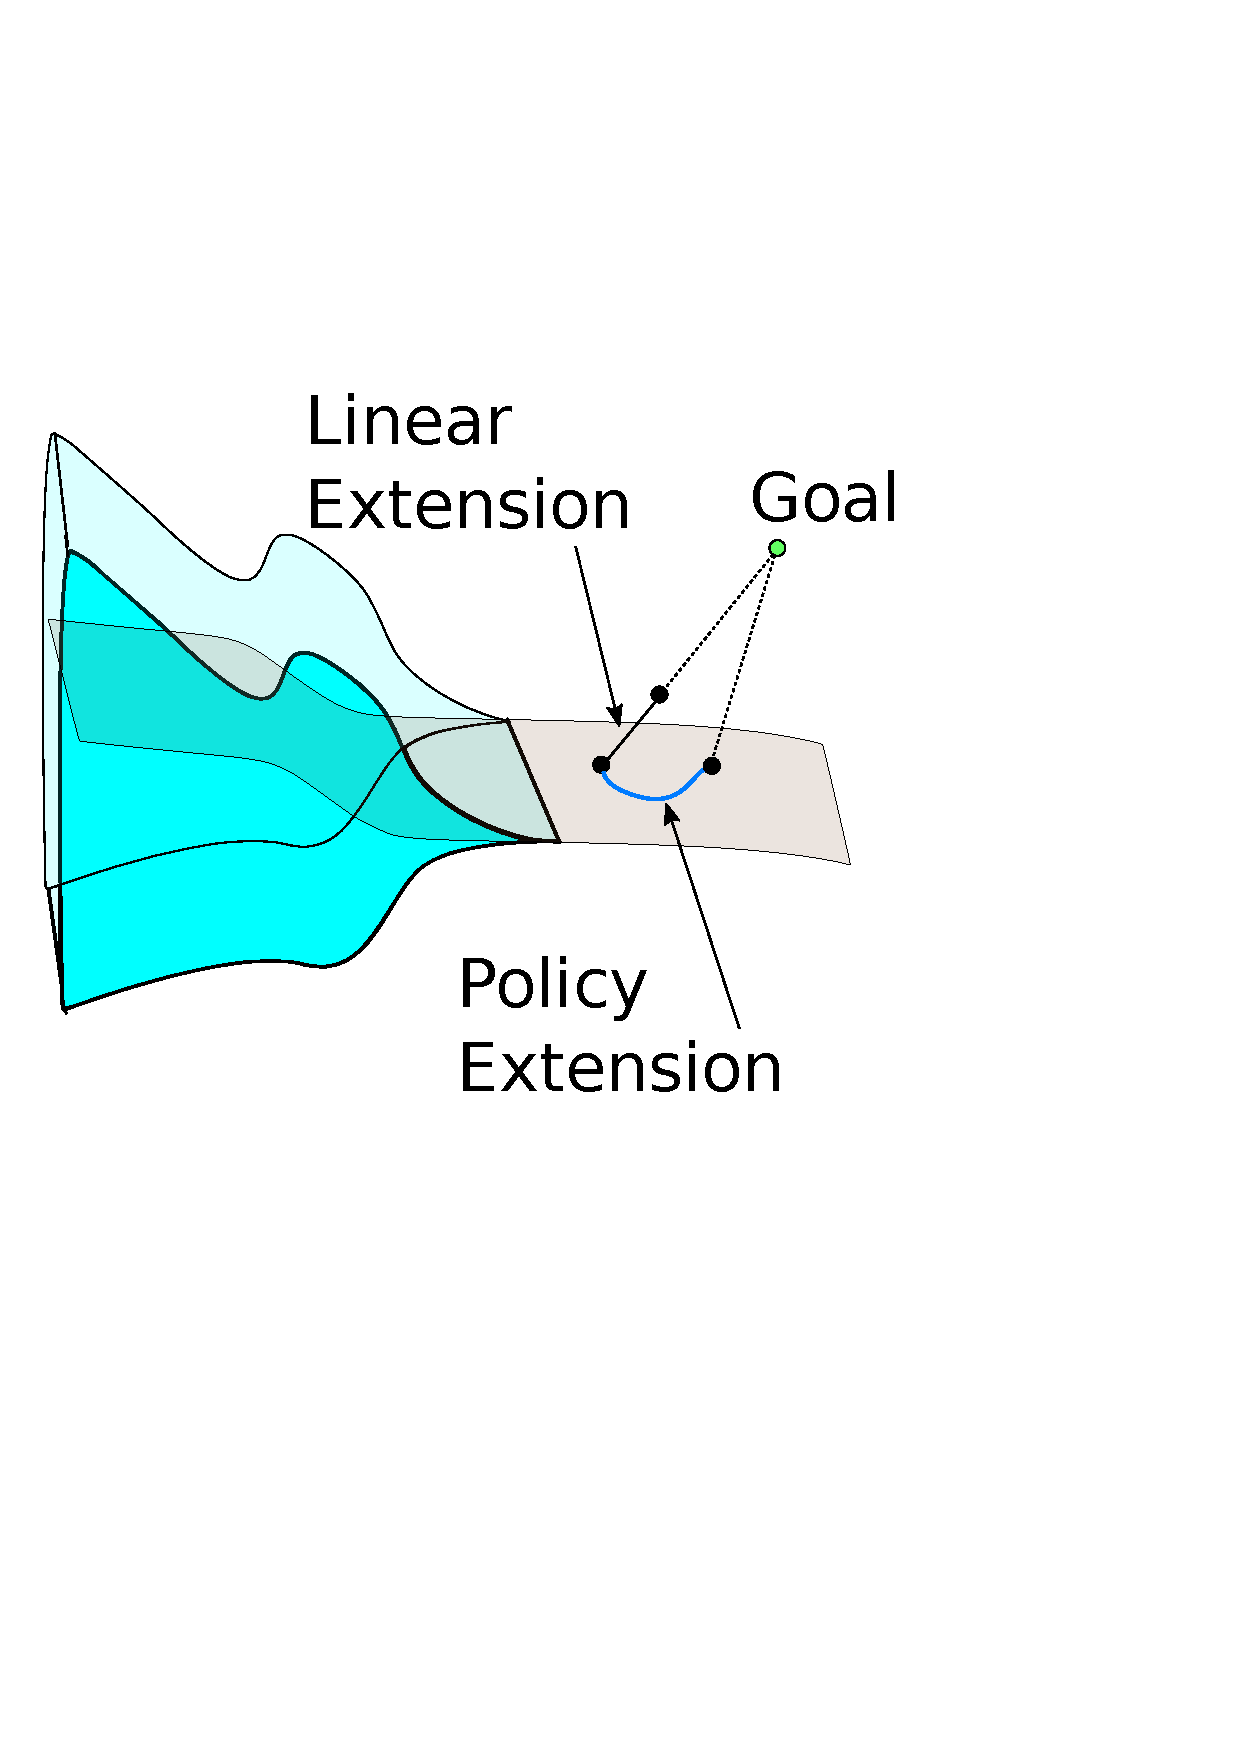
\includegraphics[width=.5\linewidth]{./Planning/extend.pdf}
  
  \caption{Illustration of Gradient RRT extension on the contact manifold}
  \label{fig:Extend}
\end{figure}


%% \section{Experiments}
%% \subsection{Simulation and Robot Model}
%% \subsection{Robot Snakes on a Plane}

\end{document}
